\newpage
%//------ Section 06 -------------------------------------------------------------------------------------------------
\section{Results}
\label{sec:Section06}
%//-----------------------------------------------------------------------//

\subsection{Experimental results}
\label{sec:Section06.a-}

\subsubsection{Sub-Sbsection}

The yield ratio distribution of \rmPhiMes and \rmOmegaPM, measured at \absrap < 0.5, is shown in \fig \ref{fig:YieldEffCorr} for the multiplicity class I. One may notice the arising of a peak around $\Delta y$ close to zero ; this suggests an increase of \rmPhiMes yield, as it gets closer to the \rmOmegaPM. 

Nevertheless, as explained in section \ref{sec:Section03}, all the \rmPhiMes within the event are paired with the trigger particle, meaning that associations of uncorrelated particles are present in \fig \ref{fig:YieldEffCorr}. Instead, one can look at the yield ratio distribution of \rmPhiMes and \rmOmegaPM with respect to the very same ratio but formed with uncorrelated pairs. The latter is obtained using an event-mixing technique, which consists in pairing \rmOmegaPM from one event with \rmPhiMes from five different events. Those events must pass the following criteria : the difference in longitudinal position of the primary vertex has to remain within $\pm$ 1 cm, and they are requiered to share the same multiplicity percentile with a tolerance of $\pm$ 10 \%. Yield ratio distribution of \rmPhiMes and \rmOmegaPM, based upon uncorrelated pairs, is depicted on \fig \ref{fig:YieldWrongPairEffCorr}.

\begin{figure}[h]
	\centering
	\begin{subfigure}[b]{.45\linewidth}
         \centering
         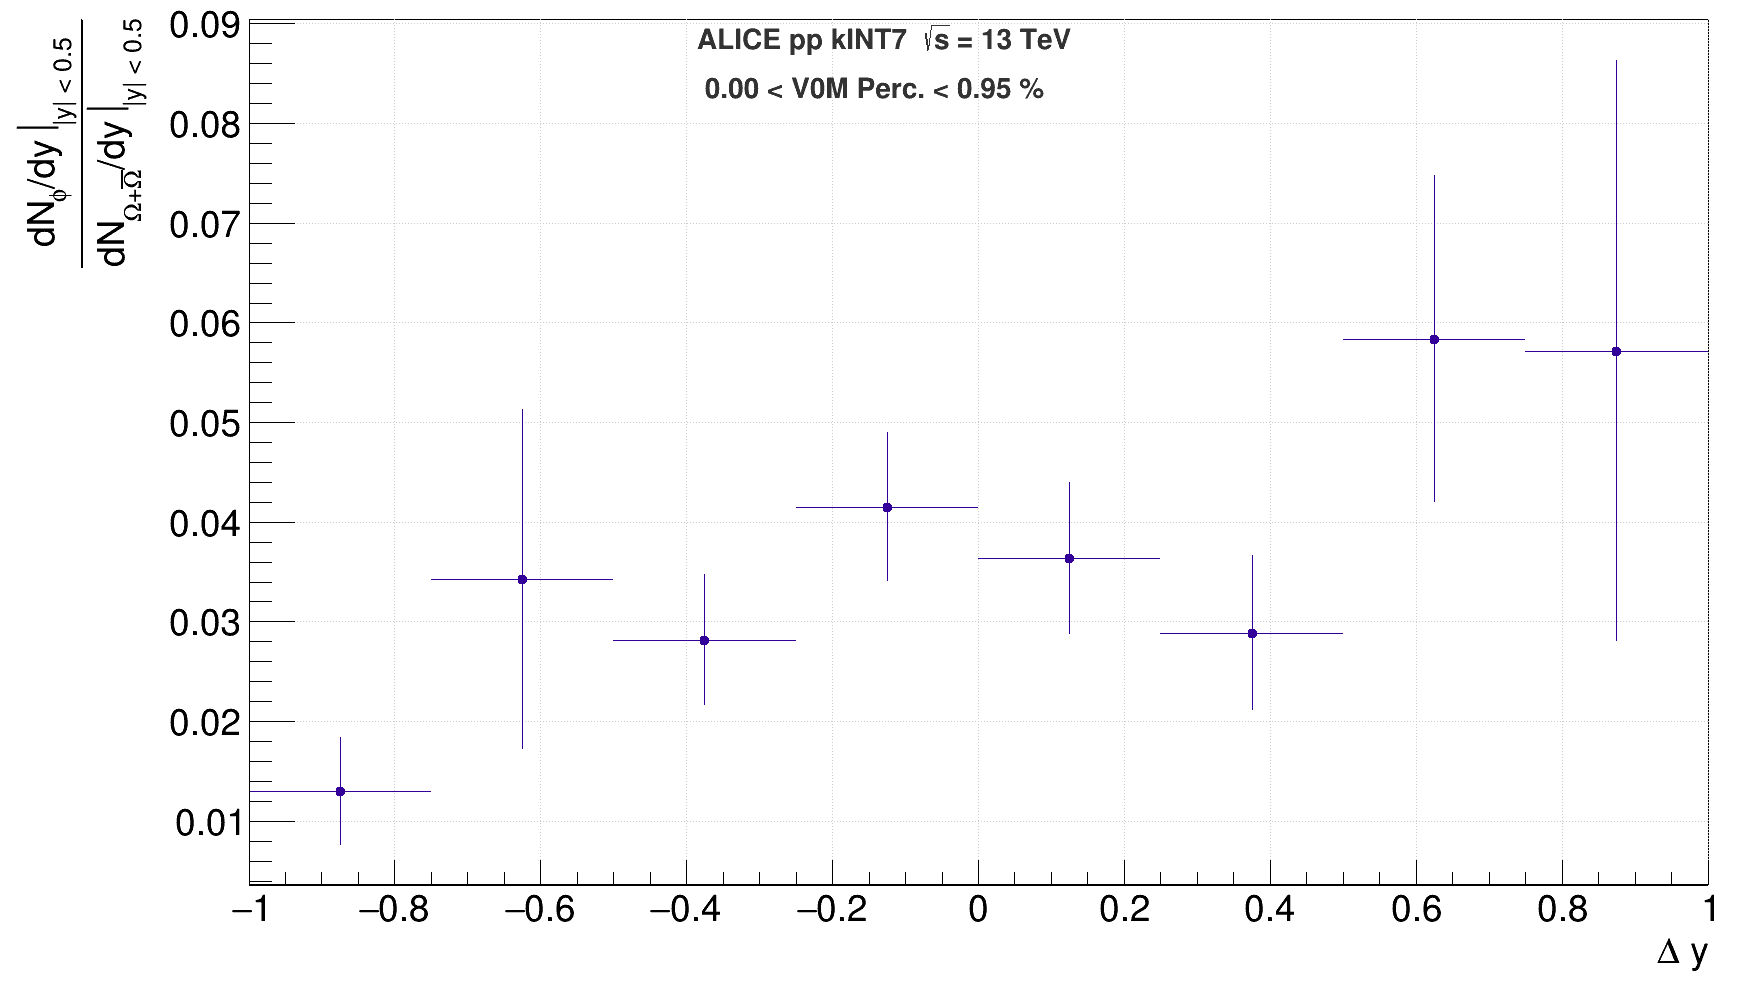
\includegraphics[width=1.\textwidth, angle=0, clip=true, trim=0cm 0 0 0]{Figures/Sec06_Results/EfficiencyCorrectedYield.png} 
         \caption{ }
         \label{fig:YieldEffCorr}
    \end{subfigure}
    \hfill
    \begin{subfigure}[b]{.45\linewidth}
         \centering
         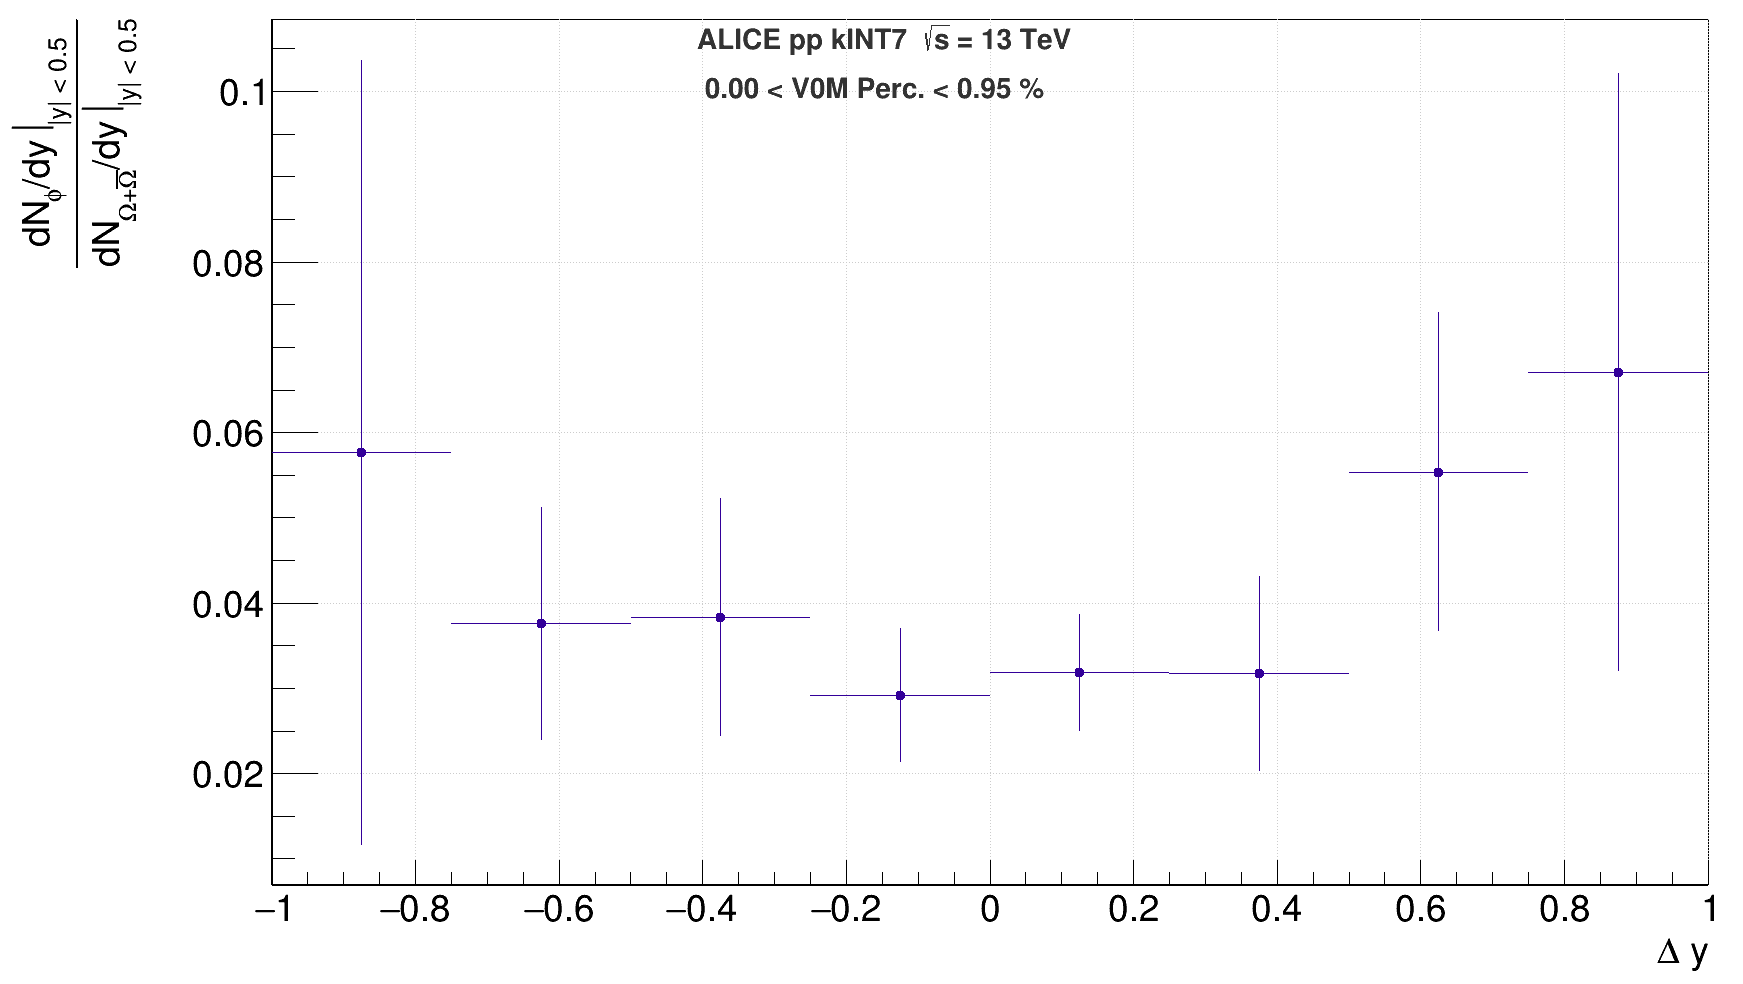
\includegraphics[width=1.\textwidth, angle=0, clip=true, trim=0cm 0 0 0cm]{Figures/Sec06_Results/WrongCorrectedYield.png}
         \caption{ }
         \label{fig:YieldWrongPairEffCorr} 
    \end{subfigure}
    \hfill
    \begin{subfigure}[b]{.45\linewidth}
         \centering
         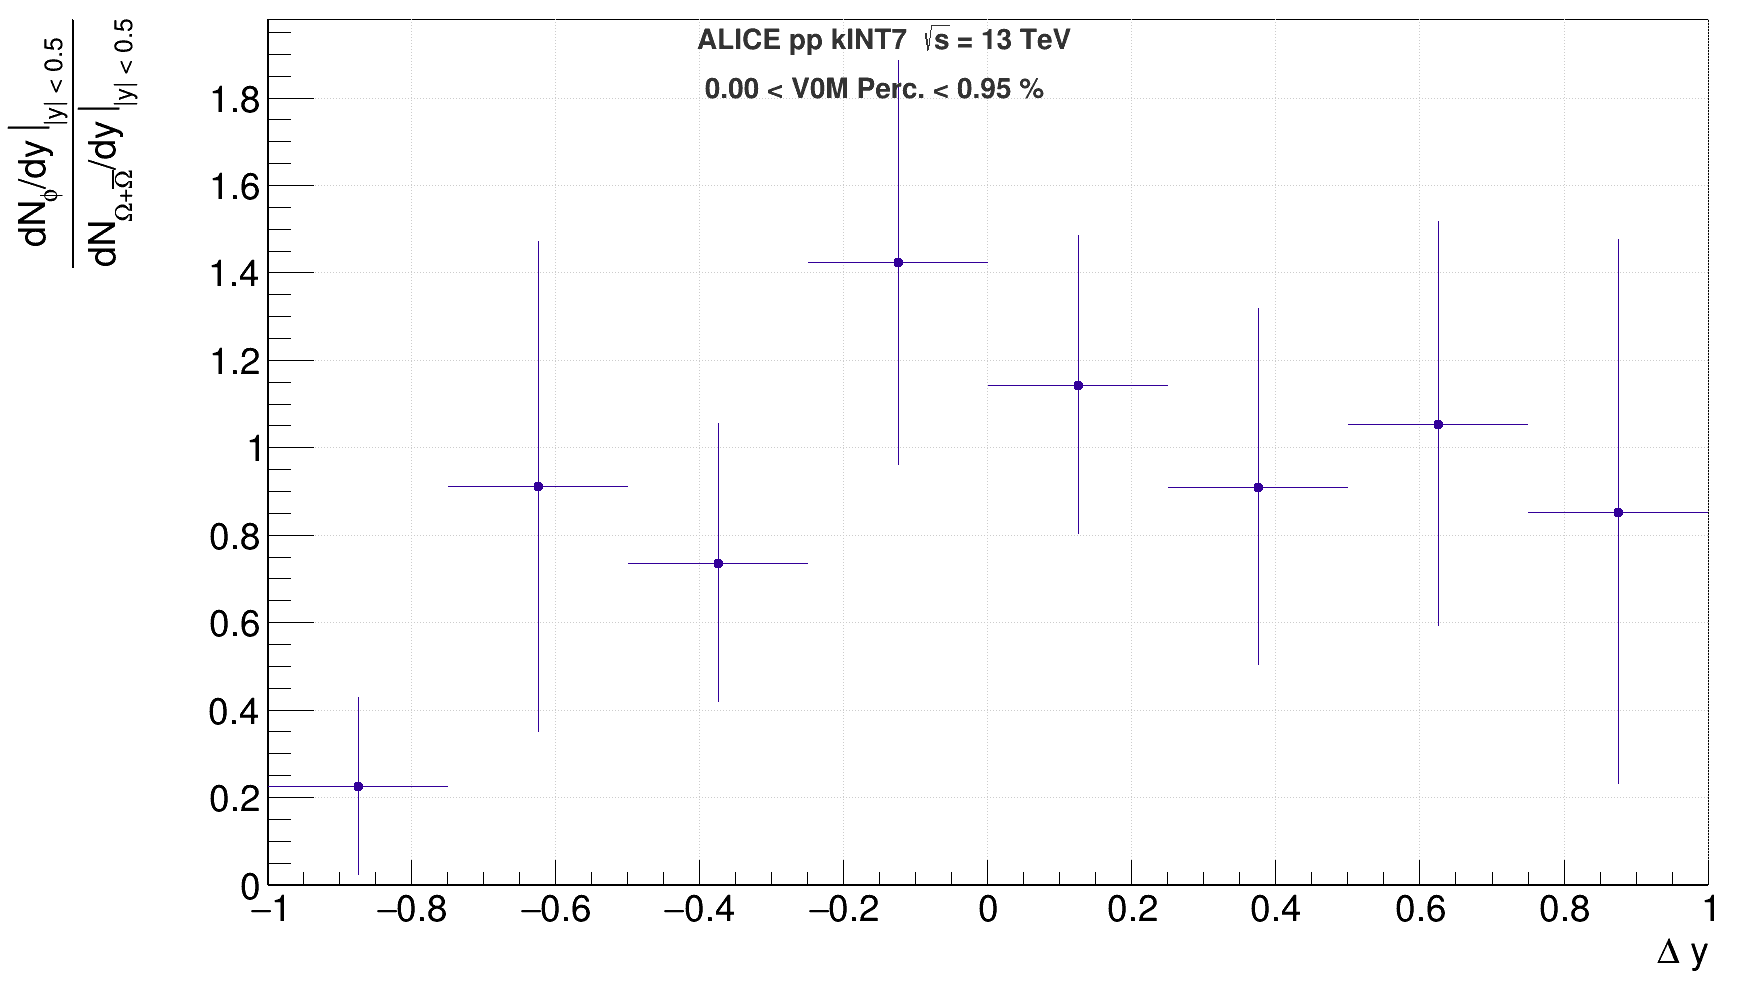
\includegraphics[width=1.\textwidth, angle=0, clip=true, trim=0cm 0 0 0cm]{Figures/Sec06_Results/Eff+PairCorrectedYield.png}
         \caption{ }
         \label{fig:YieldPair+EffCorr} 
    \end{subfigure}
\caption{Yield ratio of \rmPhiMes and (\rmOmegas), event-by-event, as a function of their difference in rapidity, $\Delta y$. \fig \ref{fig:YieldEffCorr} depicts the efficiency corrected yield ratio with same-event pairs ; both species are corrected individually. \fig \ref{fig:YieldWrongPairEffCorr} represents the efficiency corrected yield ratio with mixed-event pairs. Division of the two previous yield ratio is presented in \fig \ref{fig:YieldPair+EffCorr}, meaning the efficiency and pair acceptance corrected yield ratio.}
	\label{fig:Yield}
\end{figure}


\rmPhiMes-\rmOmegaPM pair acceptance and efficiency corrected yield distribution, measured at \absrap < 0.5, is presented on \fig \ref{fig:YieldPair+EffCorr} for class I events. A trend seems to emerge : the yield ratio increases as the \rmPhiMes gets closer to the \rmOmegaPM. Yet, this production enhancement is comprised within the error bars. It is interesting to note that the ratio is distributed around unity, meaning that the yield of \rmPhiMes is almost equal to the one of \rmOmega, whenever \rmOmega is present within the event.

\subsection{Comparison with MC models}
\label{sec:Section06.b-}